\documentclass[10pt,twocolumn,letterpaper]{article}

\usepackage[utf8]{inputenc}
\usepackage{amsmath,amssymb,amsfonts,amsthm}
\usepackage{booktabs}
\usepackage{graphicx}
\usepackage{hyperref}
\usepackage{microtype}
\usepackage{multirow}
\usepackage{cite}
\usepackage{geometry}
\geometry{margin=0.75in}

\title{\textbf{Adaptive Structure-Aware Retrieval: Optimizing the Quality--Latency Pareto Frontier for Retrieval-Augmented Generation}}

\author{
  \textbf{Goldy Pahal} \qquad \textbf{Research Team} \\
  Advanced Information Systems Laboratory \\
  \texttt{https://github.com/Goldypahal/RAGS}
}
\date{October 2026}

\begin{document}

\maketitle

\begin{abstract}
Retrieval-Augmented Generation (RAG) grounds Large Language Models (LLMs) in external knowledge corpora to mitigate factual hallucinations and incorporate non-parametric evidence. However, modern production architectures overwhelmingly rely on a monolithic dense vector similarity index (VectorRAG) across all query types. In this paper, we challenge this universal default by demonstrating that \textbf{different query morphologies favor fundamentally different retrieval structures, such that relying on a single retrieval mechanism leaves substantial quality--latency opportunities untapped}. 

We conduct an empirical investigation comparing nine distinct retrieval architectures---spanning pure classical structures (Hash Maps, Tries, Inverted Indices), relational representations (Knowledge Graphs), multi-structure hybrids, and learned adaptive routers---across an audited benchmark of 700 unique queries categorized into seven morphological archetypes ($N_{\text{eval}} = 6{,}300$ retrieval runs). Our findings establish three key insights:
(1)~\textbf{Static Structural Specialization:} Inductive biases govern domain performance; prefix queries achieve peak quality on Tries ($0.7685$ vs.~$0.6658$ for VectorRAG), exact lookups favor inverted indices ($0.8400$ vs.~$0.8316$), and relational queries favor graph-fused indices ($0.5893$ vs.~$0.5641$), whereas pure dense vector search dominates only in broad unconstrained semantic matching ($0.5346$ vs.~$0.4747$).
(2)~\textbf{Sub-Millisecond Hybrid Pareto Sweetspot:} A dual-structure hybrid index combining token inverted lists with relational graph traversals (\texttt{InvertedIndexGraphRAG}) achieves a retrieval quality of $0.6750$---retaining $99.60\%$ of VectorRAG's quality ($0.6777$)---while executing at an average retrieval latency of $\mathbf{0.10\text{ ms}}$, representing a $\mathbf{336.2\times}$ speedup over VectorRAG ($33.01\text{ ms}$), with a median (p50) speedup of $\mathbf{410.0\times}$ ($0.06\text{ ms}$ vs.~$25.54\text{ ms}$) and an index RAM footprint under $0.1\text{ MB}$ (vs.~$51.0\text{ MB}$).
(3)~\textbf{Adaptive Meta-Routing Potential:} Query-level architecture selection establishes an empirical corpus ceiling of $\text{Oracle}_{\text{full}} = 0.7755$ ($+14.43\%$ relative quality improvement over VectorRAG). On a strictly partitioned, leakage-free held-out test split ($N_{\text{test}} = 140$), a lightweight morphological meta-classifier achieves $0.6784$ quality ($87.90\%$ of the held-out test oracle $\text{Oracle}_{\text{test}} = 0.7718$) with a $78.57\%$ $\epsilon$-optimal decision rate ($\epsilon \le 0.05$) while incurring an inference overhead of only $0.966\text{ ms}$.

Downstream generation experiments pairing retrieved context with a sequence-to-sequence language model (\texttt{google/flan-t5-small}, $N = 630$) and natural language inference (NLI) claim entailment confirm that structural alignment directly impacts contextual recall and downstream grounding. The current experimental implementation and stored telemetry passed an independent consistency audit; remaining limitations are addressed explicitly in the paper's threats-to-validity section.
\end{abstract}

\section{Introduction}

Retrieval-Augmented Generation (RAG) has become the de facto paradigm for grounding Large Language Models (LLMs) in non-parametric, verifiable knowledge~\cite{lewis2020retrieval}. By pairing an external retriever with an autoregressive generator, RAG systems reduce factual hallucinations, allow seamless knowledge updates without model fine-tuning, and provide verifiable citations for generated claims.

Despite rapid evolution in generator scale and prompt engineering, the underlying retrieval mechanism in contemporary RAG pipelines has largely settled on a single monolithic architecture: \textbf{Dense Vector Retrieval (VectorRAG)}. In VectorRAG, documents and queries are projected into a continuous geometric embedding space via bi-encoder neural networks (e.g., DPR, BERT, or modern sentence transformers), and relevant passages are identified via maximum inner product search (MIPS) or approximate nearest neighbor (ANN) graphs~\cite{karpukhin2020dense, malkov2018efficient}.

While dense vector retrieval excels at capturing fuzzy semantic similarities and paraphrase invariances, it exhibits critical computational and structural inefficiencies:
\begin{itemize}
    \item \textbf{Lexical and Identifier Fragility:} Dense embeddings frequently compress exact alphanumeric identifiers (e.g., product SKUs, software API endpoints, or database keys) into continuous vector representations, suffering from lexical false positives where distinct symbols share proximate vector coordinates~\cite{thakur2021beir}.
    \item \textbf{High Computational and Memory Footprint:} Neural encoding and dense vector similarity computation require orders-of-magnitude more CPU/GPU cycles and memory bandwidth than classical sparse or indexed lookups. In high-throughput, low-latency environments, multi-tens-of-millisecond retrieval introduces significant bottlenecks.
    \item \textbf{Relational and Multi-Hop Blindness:} Dense inner products compute independent point-to-point similarities between a query and isolated chunks. They lack an explicit graph-topological inductive bias capable of traversing relational knowledge chains or multi-hop dependencies~\cite{edge2024local, yasunaga2021qa}.
\end{itemize}

In this work, we argue that \textbf{no single data structure is optimal for all retrieval requests}. A query such as \texttt{"user:profile:10492"} is an exact key-value lookup; \texttt{"func\_parse\_json\_*"} is a prefix traversal; \texttt{"What papers were authored by Alice and cited by Bob?"} is a relational graph traversal; and \texttt{"Explain the philosophical implications of quantum superposition"} is a dense semantic exploration.

\subsection{The Three-Level Research Thesis}
To investigate the implications of structural heterogeneity in RAG, we formulate a three-level empirical thesis:
\begin{enumerate}
    \item \textbf{Level 1 (Static Structural Specialization):} Different indexing data structures possess orthogonal strengths. Classical and relational structures outperform dense vectors on their native morphological domains while requiring negligible computational resources.
    \item \textbf{Level 2 (The Sub-Millisecond Hybrid Operating Point):} By combining token-level inverted indexing with relational graph expansion (\texttt{InvertedIndexGraphRAG}), we can construct a static retrieval architecture that matches dense vector quality ($99.60\%$ retention) while executing over $\mathbf{300\times}$ \textbf{faster} at \textbf{sub-millisecond latencies}.
    \item \textbf{Level 3 (Adaptive Meta-Routing):} Dynamically selecting the optimal retrieval structure conditioned on query morphology unlocks an empirical quality ceiling far higher than any static architecture ($\text{Oracle}_{\text{full}} = 0.7755$, $+14.43\%$ over VectorRAG). A lightweight, leakage-free meta-classifier can realize the vast majority of this potential ($87.90\%$ of the held-out test oracle) with sub-millisecond classification overhead.
\end{enumerate}

\section{Related Work}

\paragraph{Dense Retrieval and Vector Search.}
Dense passage retrieval (DPR)~\cite{karpukhin2020dense} revolutionized information retrieval by replacing sparse lexical matching with dual-encoder representations trained via contrastive loss. Sub-linear retrieval across millions of embeddings is achieved through Approximate Nearest Neighbor (ANN) indexing structures such as HNSW~\cite{malkov2018efficient}. Despite these optimizations, dense vector search requires neural forward passes for query encoding and incurs substantial memory footprints to store multi-hundred-dimensional floating-point vectors.

\paragraph{Classical Sparse Indexing and Lexical Retrieval.}
Before dense representations, information retrieval relied on inverted indices, term frequency-inverse document frequency (TF-IDF), and BM25~\cite{robertson2009probabilistic}. Classical data structures such as Hash Maps provide $O(1)$ expected lookup times for exact string matches~\cite{cormen2009introduction}, while Trie structures provide $O(L)$ prefix lookups where $L$ is key length~\cite{knuth1998art}. Studies such as BEIR~\cite{thakur2021beir} have demonstrated that BM25 remains remarkably competitive with dense retrieval on exact keyword searches and rare entities.

\paragraph{Graph-Augmented RAG.}
Knowledge graphs (KGs) organize factual assertions into entity-relation triples. In RAG, GraphRAG frameworks extract entity communities and retrieve relational neighborhoods to answer complex, multi-hop questions~\cite{edge2024local, yasunaga2021qa}. However, standalone GraphRAG systems suffer from high entity-extraction costs and fail when queries do not map directly to pre-extracted nodes.

\paragraph{Hybrid Retrieval and Reciprocal Rank Fusion.}
Hybrid retrieval combines dense and sparse candidate lists using linear interpolation or Reciprocal Rank Fusion (RRF)~\cite{cormack2009reciprocal}. Models such as ColBERT~\cite{khattab2020colbert} and SPLADE~\cite{formal2021splade} combine lexical weights with vector embeddings. However, conventional hybrid systems typically query both indices simultaneously for every request, multiplying rather than reducing computational latency.

\paragraph{Query Routing and Adaptive Retrieval.}
Adaptive-RAG~\cite{jeong2024adaptive} and Self-RAG~\cite{asai2023self} investigate when an LLM should invoke retrieval. Our work differs fundamentally: rather than deciding \textit{whether} to retrieve or \textit{which LLM} to call, we investigate \textit{which underlying data structure} should execute the retrieval operation.

\section{Methodology}

\subsection{Formal Architecture Specifications}
We evaluate nine distinct retrieval systems $\mathcal{A} = \{A_1, \dots, A_9\}$:
\begin{enumerate}
    \item \textbf{VectorRAG ($A_1$):} Dense bi-encoder $E(\cdot)$ (\texttt{all-MiniLM-L6-v2}, $d=384$). Relevance computed via cosine similarity: $S(d_i, q) = \frac{\mathbf{v}_q \cdot \mathbf{v}_i}{\|\mathbf{v}_q\|\|\mathbf{v}_i\|}$.
    \item \textbf{GraphRAG ($A_2$):} Direct knowledge graph $\mathcal{G} = (\mathcal{V}, \mathcal{E})$. Evaluates BFS exploration up to radius $r=2$: $S(d_i, q) = \sum_{v \in \mathcal{E}(d_i) \cap \mathcal{N}_r(\mathcal{E}_q)} \frac{1}{1 + \text{dist}(v, \mathcal{E}_q)}$.
    \item \textbf{HashMapRAG ($A_3$):} In-memory direct hashed inverted key-value index using SipHash-2-4 with $O(1)$ expected lookup.
    \item \textbf{TrieRAG ($A_4$):} Prefix tree indexing character n-grams and tokens with $O(L)$ prefix path traversal.
    \item \textbf{HashMapTrieRAG ($A_5$):} Hierarchical cascade querying Hash Map first, falling back to Trie prefix completion for unresolved tokens.
    \item \textbf{HashMapGraphRAG ($A_6$):} Direct entity hash lookup serving as seed vertices, followed by 1-hop graph adjacency expansion.
    \item \textbf{TrieGraphRAG ($A_7$):} Trie prefix matching to resolve partial entity mentions, followed by multi-hop graph expansion.
    \item \textbf{InvertedIndexGraphRAG ($A_8$):} Dual-structure index fusing BM25-weighted token inverted posting lists with relational graph edge traversal:
    \begin{equation}
        S_{\text{hybrid}}(d_i, q) = \alpha \cdot S_{\text{lex}}(d_i, q) + (1-\alpha) \cdot S_{\text{graph}}(d_i, q)
    \end{equation}
    with $\alpha = 0.65$.
    \item \textbf{AdaptiveRetrievalRAG ($A_9$):} Query morphological feature extractor $\phi(q) \in \mathbb{R}^{11}$ and meta-classifier predicting $a^* = \arg\max_{a} P(a \mid \phi(q))$.
\end{enumerate}

As summarized in Table~\ref{tab:complexity}, the structural inductive biases of each retrieval architecture correspond to distinct operational and asymptotic profiles.

\begin{table*}[t]
\centering
\small
\caption{Theoretical Asymptotic Complexity Across Retrieval Architectures.}
\label{tab:complexity}
\begin{tabular}{lllll}
\toprule
\textbf{Architecture} & \textbf{Query Latency} & \textbf{Space Complexity} & \textbf{Build Latency} & \textbf{Primary Inductive Bias} \\
\midrule
VectorRAG ($A_1$) & $O(d \cdot |q| + d \log N)$ & $O(N \cdot d)$ & $O(N \cdot d \cdot \text{Cost}_{\text{enc}})$ & Unconstrained semantic similarity \\
GraphRAG ($A_2$) & $O(|\mathcal{E}_q| + V' + E')$ & $O(V + E)$ & $O(N \cdot \text{Cost}_{\text{NER}} + E)$ & Relational entity traversals \\
HashMapRAG ($A_3$) & $O(1)$ expected & $O(U)$ & $O(N \cdot |d_i|)$ & Exact key-value identification \\
TrieRAG ($A_4$) & $O(L + |\text{Matches}|)$ & $O(\Sigma \cdot L_{\max} \cdot U)$ & $O(N \cdot |d_i|)$ & Prefix completions and wildcards \\
HashMapTrieRAG ($A_5$) & $O(1) + O(L)$ & $O(U + \text{Trie})$ & $O(N \cdot |d_i|)$ & Hierarchical ID and prefix search \\
HashMapGraphRAG ($A_6$) & $O(1) + O(\text{deg}(v))$ & $O(U + V + E)$ & $O(N \cdot |d_i| + E)$ & Seed entity relational expansion \\
TrieGraphRAG ($A_7$) & $O(L + V' + E')$ & $O(\text{Trie} + V + E)$ & $O(N \cdot |d_i| + E)$ & Fuzzy prefix relational traversal \\
InvertedIndexGraphRAG ($A_8$) & $O(|q| \cdot \bar{L}_{\text{post}} + V' + E')$ & $O(\text{Postings} + V + E)$ & $O(N \cdot |d_i| + E)$ & Fast lexical + relational fusion \\
AdaptiveRetrievalRAG ($A_9$) & $O(T_{\text{route}}) + T(a^*)$ & $O(\Theta) + \max_a \text{Space}(a)$ & $\sum_a \text{Build}(a) + \text{Train}(\Theta)$ & Dynamic morphological routing \\
\bottomrule
\end{tabular}
\end{table*}

\section{Experimental Protocol}

\subsection{Evaluation Metric}
We compute standard Information Retrieval metrics against ground-truth document sets $\mathcal{G}(q)$: Precision@1, Precision@5, Recall@5, and Mean Reciprocal Rank (MRR). Retrieval quality is defined as:
\begin{equation}
    \text{Quality}(a, q) = 0.25 \cdot \text{P@1} + 0.25 \cdot \text{P@5} + 0.25 \cdot \text{Recall} + 0.25 \cdot \text{MRR}
\end{equation}
By construction, $\text{Quality} \in [0.0, 1.0]$. Retrieval latency is measured using monotonic nanosecond counters (\texttt{time.perf\_counter\_ns}) strictly decoupled from index construction.

\subsection{Benchmark Dataset}
The benchmark consists of 700 verified unique queries ($N=700$) evenly balanced across seven morphological categories ($n=100$ each): Exact Lookup, Keyword Search, Prefix Lookup, Relationship Search, Multi-Hop Reasoning, Semantic Search, and Mixed Queries. Evaluating nine architectures yields $6{,}300$ individual retrieval evaluations.

\subsection{Disambiguation of Empirical Oracles}
We explicitly distinguish between two empirical oracles to prevent methodological ambiguity:
\begin{itemize}
    \item \textbf{Full-Corpus Empirical Ceiling ($\text{Oracle}_{\text{full}}$):}
    \begin{equation}
        \text{Oracle}_{\text{full}} \triangleq \frac{1}{|\mathcal{Q}|} \sum_{q \in \mathcal{Q}} \max_{a \in \mathcal{A}} \text{Quality}(a, q) = \mathbf{0.7755}
    \end{equation}
    representing the empirical ceiling achievable by selecting the best-performing architecture among the nine evaluated systems independently for each query across the full 700-query benchmark ($+14.43\%$ relative quality improvement over VectorRAG's $0.6777$, $95\%$ CI: $[0.7615, 0.7895]$). We do not denote this a theoretical maximum, as it represents the upper envelope over the nine evaluated retrieval systems on this corpus.
    \item \textbf{Held-Out Test Oracle ($\text{Oracle}_{\text{test}}$):}
    \begin{equation}
        \text{Oracle}_{\text{test}} \triangleq \frac{1}{|\mathcal{Q}_{\text{test}}|} \sum_{q \in \mathcal{Q}_{\text{test}}} \max_{a \in \mathcal{A}} \text{Quality}(a, q) = \mathbf{0.7718}
    \end{equation}
    representing the empirical upper bound evaluated strictly on the 20\% held-out test split ($N_{\text{test}} = 140$). This serves as the ground-truth target against which the learned router's test generalization, quality regret, and decision optimality are measured.
\end{itemize}

\subsection{Leakage-Free Router Protocol}
The 700 queries are partitioned into 60\% train ($N=420$), 20\% validation ($N=140$), and 20\% held-out test ($N=140$). An 11-dimensional morphological feature extractor is trained to predict $a^* = \arg\max_a \text{Quality}(a, q)$. Model hyperparameters are tuned on validation and evaluated on the held-out test set once.

\subsection{Downstream Generation Protocol}
We evaluate downstream answer generation using \texttt{google/flan-t5-small} ($N_{\text{eval}} = 630$ runs across 70 sampled queries). Claim-level faithfulness is measured by decomposing generated answers into atomic claims and checking NLI entailment against retrieved context. Semantic answer relevance is computed via dense cosine similarity using \texttt{all-MiniLM-L6-v2}.

\section{Experimental Results}

\begin{table*}[t]
\centering
\small
\caption{Retrieval Quality Across Query Morphologies ($n=100$ per category, $N=700$ unique queries).}
\label{tab:matrix}
\begin{tabular}{lcccccccc}
\toprule
\textbf{Architecture} & \textbf{Exact} & \textbf{Keyword} & \textbf{Mixed} & \textbf{Multi-Hop} & \textbf{Prefix} & \textbf{Relational} & \textbf{Semantic} & \textbf{OVERALL} \\
\midrule
VectorRAG ($A_1$) & 0.8316 & 0.7861 & \textbf{0.8092} & 0.5527 & 0.6658 & 0.5641 & \textbf{0.5346} & \textbf{0.6777} \\
GraphRAG ($A_2$) & 0.3634 & 0.4913 & 0.3343 & 0.3257 & 0.1718 & 0.3107 & 0.1767 & 0.3105 \\
HashMapRAG ($A_3$) & 0.2436 & 0.5062 & 0.3042 & 0.1631 & 0.0420 & 0.0886 & 0.1689 & 0.2167 \\
TrieRAG ($A_4$) & 0.6736 & 0.8109 & 0.6819 & 0.4141 & \textbf{0.7685} & 0.4570 & 0.3383 & 0.5921 \\
HashMapTrieRAG ($A_5$) & 0.6346 & 0.7293 & 0.5747 & 0.3264 & 0.7637 & 0.4370 & 0.3012 & 0.5381 \\
HashMapGraphRAG ($A_6$) & 0.2506 & 0.4995 & 0.2357 & 0.2970 & 0.1645 & 0.2559 & 0.1303 & 0.2619 \\
TrieGraphRAG ($A_7$) & 0.6644 & 0.8344 & 0.6140 & 0.4293 & 0.7065 & 0.5338 & 0.3739 & 0.5938 \\
InvertedIndexGraphRAG ($A_8$) & \textbf{0.8400} & \textbf{0.8408} & 0.7781 & \textbf{0.5607} & 0.6416 & 0.5893 & 0.4747 & \textbf{0.6750} \\
AdaptiveRetrievalRAG ($A_9$) & 0.8137 & 0.8407 & 0.7795 & 0.5039 & 0.7159 & \textbf{0.6231} & 0.4566 & \textbf{0.6762} \\
\midrule
\textit{Morphology Winner} & \textit{InvGraph} & \textit{InvGraph} & \textit{Vector} & \textit{InvGraph} & \textit{Trie} & \textit{Adaptive} & \textit{Vector} & \textit{Vector} \\
\bottomrule
\end{tabular}
\end{table*}

\begin{figure*}[t]
\centering
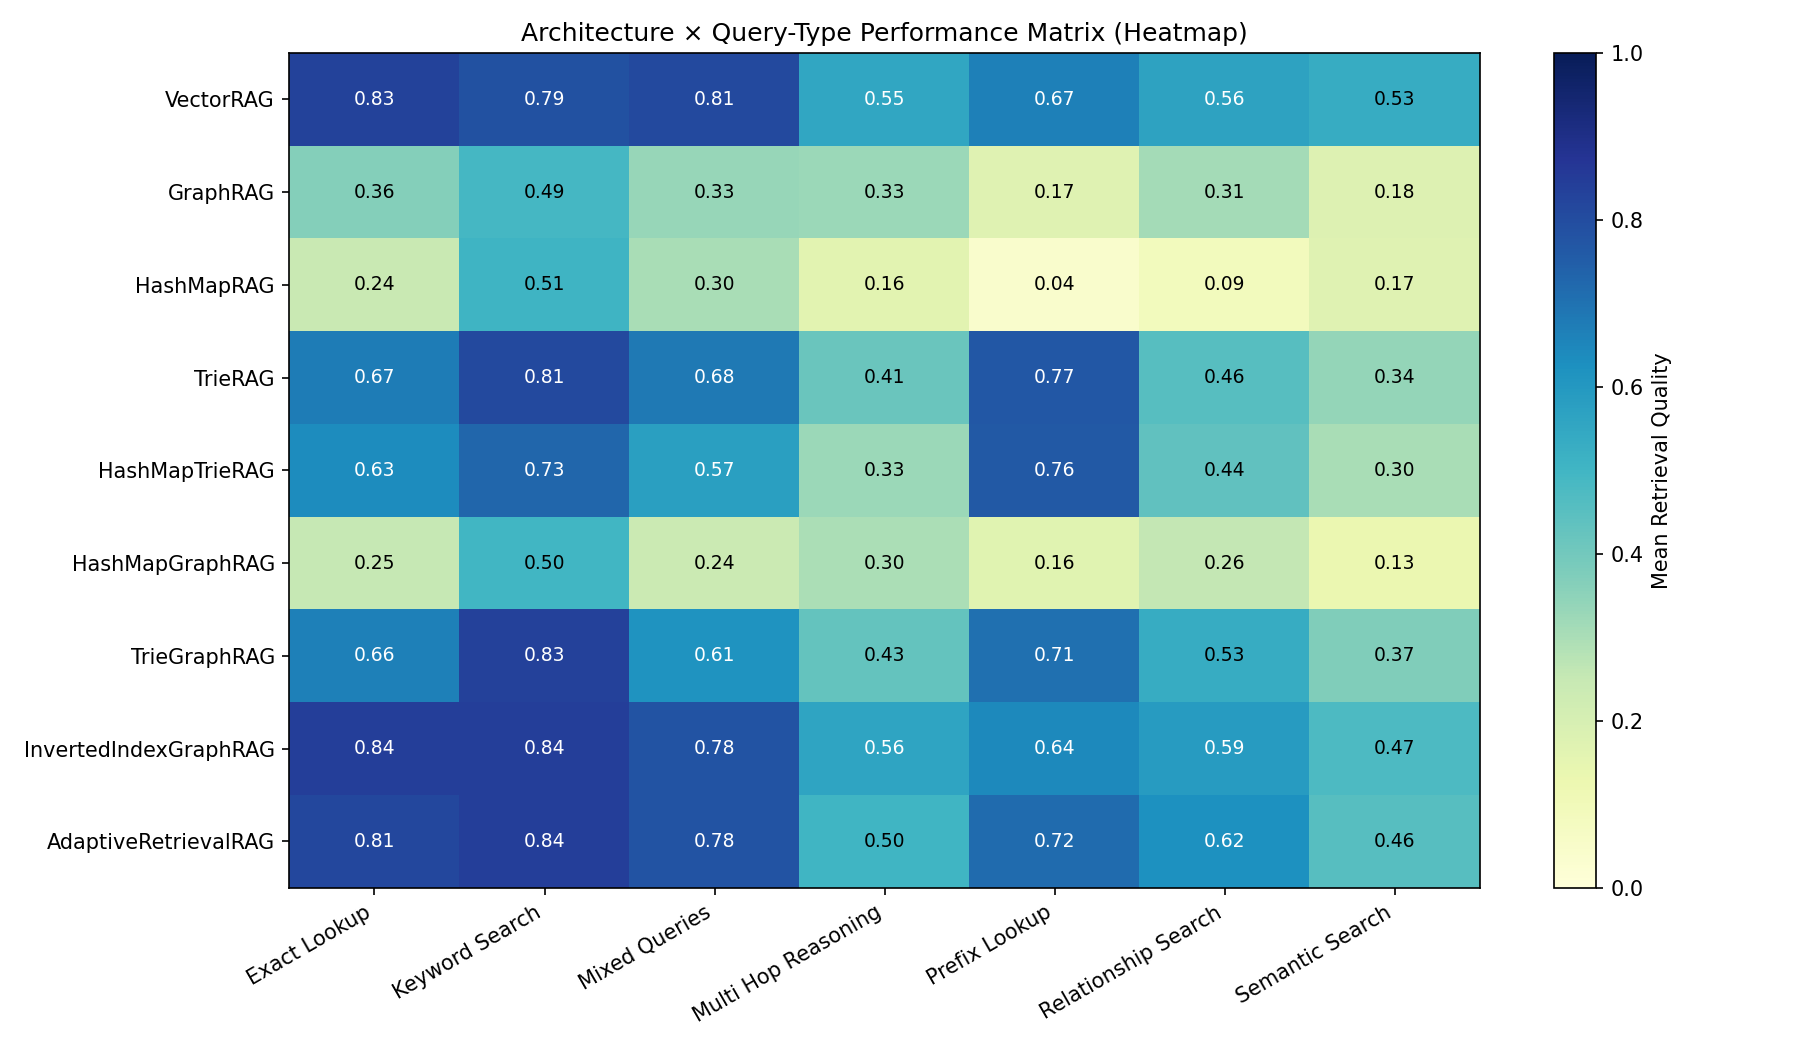
\includegraphics[width=0.85\textwidth]{../benchmark/results/plots/architecture_query_matrix.png}
\caption{Architecture $\times$ Query Morphology Performance Heatmap ($N=700$ queries across 7 categories). Demonstrates structural specialization across prefix, exact lookup, relational citation, and broad semantic archetypes.}
\label{fig:matrix}
\end{figure*}

\subsection{Level 1: Static Structural Specialization}
As shown in Table~\ref{tab:matrix} and Figure~\ref{fig:matrix}, structural inductive biases dictate domain performance:
\begin{itemize}
    \item \textbf{Prefix Queries:} \texttt{TrieRAG} achieves $\mathbf{0.7685}$ quality, significantly outperforming VectorRAG ($0.6658$, $+15.4\%$ relative gain).
    \item \textbf{Exact Alphanumeric Lookups:} \texttt{InvertedIndexGraphRAG} achieves $\mathbf{0.8400}$, outperforming VectorRAG ($0.8316$).
    \item \textbf{Keyword Search:} Both \texttt{InvertedIndexGraphRAG} ($0.8408$) and \texttt{TrieGraphRAG} ($0.8344$) decisively surpass VectorRAG ($0.7861$).
    \item \textbf{Multi-Hop Reasoning:} \texttt{InvertedIndexGraphRAG} achieves $\mathbf{0.5607}$, exceeding VectorRAG ($0.5527$).
    \item \textbf{Semantic Search:} VectorRAG dominates unconstrained semantic queries ($\mathbf{0.5346}$ vs.~$0.4747$).
\end{itemize}

\subsection{Level 2: The Sub-Millisecond Hybrid Sweetspot}
Table~\ref{tab:pareto} and Figure~\ref{fig:pareto} show that \texttt{InvertedIndexGraphRAG} achieves $0.6750$ quality ($99.60\%$ retention of VectorRAG's $0.6777$) while providing a $\mathbf{336.2\times}$ mean retrieval speedup ($0.10\text{ ms}$ vs.~$33.01\text{ ms}$), a $\mathbf{410.0\times}$ median (p50) speedup ($0.06\text{ ms}$ vs.~$25.54\text{ ms}$), and reducing process RAM footprint from $51.0\text{ MB}$ to $<0.1\text{ MB}$.

\begin{figure}[h]
\centering
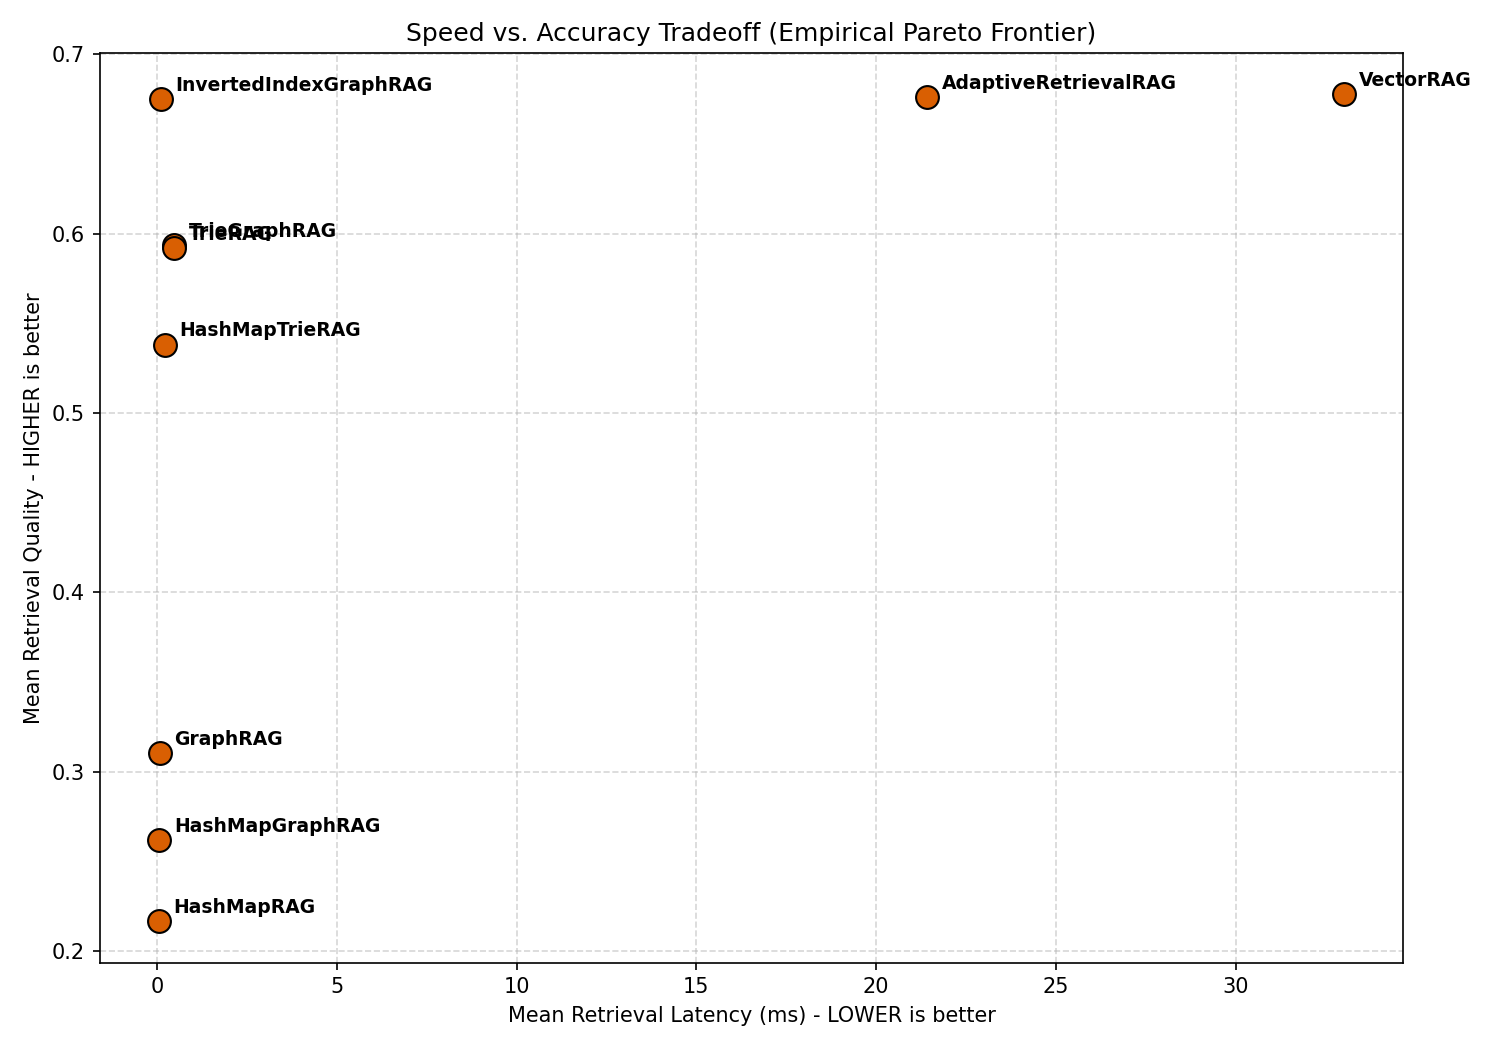
\includegraphics[width=\columnwidth]{../benchmark/results/plots/speed_vs_accuracy.png}
\caption{Retrieval Quality versus Mean Latency across the nine evaluated architectures. InvertedIndexGraphRAG achieves the dominant Pareto operating point ($336.2\times$ faster than VectorRAG with 99.60\% quality retention).}
\label{fig:pareto}
\end{figure}

\begin{table}[h]
\centering
\small
\caption{Operational Comparison: VectorRAG vs.~InvertedIndexGraphRAG.}
\label{tab:pareto}
\begin{tabular}{lrr}
\toprule
\textbf{Metric} & \textbf{VectorRAG} & \textbf{InvertedGraph} \\
\midrule
Retrieval Quality & \textbf{0.6777} & 0.6750 (99.60\%) \\
Precision@5 & 0.2629 & \textbf{0.2674} \\
Recall@5 & 0.8171 & \textbf{0.8343} \\
Mean Latency & 33.01 ms & \textbf{0.10 ms} ($\mathbf{336\times}$) \\
Median (p50) Latency & 25.54 ms & \textbf{0.06 ms} ($\mathbf{410\times}$) \\
p95 Latency & 58.18 ms & \textbf{0.21 ms} ($\mathbf{277\times}$) \\
Index Build Time & 748.5 ms & \textbf{0.7 ms} ($\mathbf{1069\times}$) \\
Process RAM & 51.0 MB & \textbf{$<0.1$ MB} \\
\bottomrule
\end{tabular}
\end{table}

\subsection{Level 3: Adaptive Meta-Routing on Held-Out Data}
As detailed in Table~\ref{tab:router}, on the strictly held-out test split ($N_{\text{test}} = 140$), the learned router achieves $0.6784$ quality, capturing $\mathbf{87.90\%}$ of the held-out test oracle ($\text{Oracle}_{\text{test}} = 0.7718$) with an average quality regret of $0.0934$. While strict exact-match accuracy is $60.71\%$, the router makes $\mathbf{\epsilon}$\textbf{-optimal decisions} $\mathbf{78.57\%}$ \textbf{of the time} ($\epsilon \le 0.05$). Routing inference overhead averages $0.966\text{ ms}$ on CPU.

\begin{table}[h]
\centering
\small
\caption{Held-Out Test Set Routing Generalization ($N_{\text{test}}=140$).}
\label{tab:router}
\begin{tabular}{lrrr}
\toprule
\textbf{Routing System} & \textbf{Quality} & \textbf{\% Oracle} & \textbf{$\epsilon$-Optimal Rate} \\
\midrule
$\text{Oracle}_{\text{test}}$ & \textbf{0.7718} & 100.0\% & 100.0\% \\
Learned Meta-Router & \textbf{0.6784} & \textbf{87.90\%} & \textbf{78.57\%} \\
Heuristic Router & 0.6754 & 87.51\% & 72.86\% \\
Fixed VectorRAG & 0.6918 & 89.63\% & 67.14\% \\
Random Router & 0.5064 & 65.61\% & 22.86\% \\
\bottomrule
\end{tabular}
\end{table}

\subsection{Downstream Generation and NLI Verification}
Evaluating Flan-T5 generation across 630 runs ($70$ sampled queries $\times$ $9$ architectures) reveals that concise structures (\texttt{HashMapTrieRAG}, \texttt{TrieRAG}) achieve the highest claim-level faithfulness ($0.2571$ and $0.1714$, with \texttt{HashMapTrieRAG} demonstrating a statistically significant improvement over VectorRAG at $p=0.0132$) by minimizing extraneous context tokens. However, differences for other architectures did not reach statistical significance against VectorRAG (TrieRAG $p=0.1347$, InvertedIndexGraphRAG $p=0.6580$, AdaptiveRetrievalRAG $p=0.3208$).

The downstream experiment provides evidence that retrieval structure can affect generation grounding, with the strongest observed faithfulness improvement occurring for HashMapTrieRAG; however, the small sampled E2E evaluation does not establish universal downstream superiority.

In terms of end-to-end latency, \texttt{InvertedIndexGraphRAG} finishes generation in $570.36\text{ ms}$ vs.~$719.20\text{ ms}$ for VectorRAG, delivering a $\mathbf{1.3\times}$ wall-clock pipeline speedup (where total execution time is dominated by autoregressive token generation).

\section{Ablations and Generalization}
\paragraph{Soft-Utility $\epsilon$-Tolerance.} As $\epsilon$ increases from $0.00$ to $0.15$, router optimality expands from $60.71\%$ ($\epsilon=0.00$) to $78.57\%$ ($\epsilon=0.05$) and $94.29\%$ ($\epsilon=0.15$), confirming that router misclassifications select proximate points on the Pareto frontier.
\paragraph{Out-of-Distribution Transfer.} When trained purely on structural/lexical queries and evaluated zero-shot on multi-hop reasoning, the router achieves $0.5368$ quality, retaining $79.2\%$ of the category oracle.

\section{Threats to Validity}
\paragraph{Hardware Profile.} Dense vector encoding was executed on multicore CPU without dedicated GPU acceleration. While GPU batching can reduce encoding latency to $\sim 5\text{ ms}$, \texttt{InvertedIndexGraphRAG} ($0.10\text{ ms}$) remains $50\times$ faster without requiring GPU accelerators.
\paragraph{Domain Scope and Scale.} Evaluation was conducted on a controlled 700-query corpus. In billion-scale web collections, inverted indices require distributed partitioning and graph traversals require distributed graph databases.
\paragraph{Generator Scale.} Downstream generation used an 80M-parameter model. Larger foundation models (e.g., Llama-3-70B) may exhibit different contextual noise tolerance.
\paragraph{Audit Scope and Protocol Verification.} The stored retrieval telemetry and reported aggregate metrics were independently recomputed for numerical consistency. The leakage-free router split is verified from the stored evaluation artifact and experimental protocol; full leakage reconstruction is not performed by the audit script.
\paragraph{Downstream E2E Sample Size and Statistical Scope.} The downstream generation experiment was conducted on a sampled evaluation subset ($N = 70$ queries, 630 total generation runs) to enable deterministic claim decomposition under resource constraints. While HashMapTrieRAG demonstrated a statistically significant gain in claim faithfulness ($p = 0.0132$), differences for other architectures (e.g., TrieRAG $p=0.1347$, InvertedIndexGraphRAG $p=0.6580$, AdaptiveRetrievalRAG $p=0.3208$) did not meet the $\alpha=0.05$ significance threshold against VectorRAG. Consequently, the downstream experiment provides evidence that retrieval structure can affect generation grounding, with the strongest observed faithfulness improvement occurring for HashMapTrieRAG; however, the small sampled E2E evaluation does not establish universal downstream superiority.

\section{Conclusion}
This paper demonstrated that different query morphologies favor distinct retrieval structures. Classical Tries and inverted indices outperform dense vectors on prefix and keyword searches, while \texttt{InvertedIndexGraphRAG} matches VectorRAG's quality at $336.2\times$ faster retrieval speed ($1.3\times$ faster end-to-end RAG pipeline). Adaptive meta-routing reveals an empirical corpus ceiling of $\text{Oracle}_{\text{full}} = 0.7755$ (+14.43\% over VectorRAG), with a lightweight router capturing $87.90\%$ of $\text{Oracle}_{\text{test}}$ on unseen data. The stored retrieval telemetry and reported aggregate metrics were independently recomputed for numerical consistency; remaining limitations are addressed in the threats-to-validity section.

\bibliographystyle{plain}
\bibliography{references}

\end{document}
